%\documentclass[a4paper,doc]{apa6}
\documentclass[a4paper]{article}
% \graphicspath{{/figures/}{./../figures/}}

\usepackage[english]{babel}
\usepackage[utf8x]{inputenc}
\usepackage{apacite}
\usepackage{authblk}  % for authors
\usepackage{xcolor}
\definecolor{mypink}{RGB}{255, 230, 255}

\usepackage{amsmath}
\usepackage{graphicx}
\usepackage{chngcntr} % appendix references
\usepackage[colorinlistoftodos,prependcaption]{todonotes}
\usepackage{pgfplotstable}
\pgfplotstableset{
	fixed zerofill,
	precision=3,
	col sep = comma,
	search path={../tables/}
}
\pgfkeys{/pgf/number format/precision=2, /pgf/number format/fixed}%

\newcommand{\getValue}[3]{%
	\pgfplotstablegetelem{#1}{#2}\of{#3}%
	\pgfmathprintnumber{\pgfplotsretval}%
}
\newcommand{\getCI}[2]{[\getValue{#1}{Lower}{#2}, \getValue{#1}{Upper}{#2}]}

\usepackage{tikz}
\usepackage{tikzscale}

\newcommand{\EJ}[1]{\todo[inline, color=green]{  #1 }}
\newcommand{\Q}[1]{\todo[inline, color=yellow]{  #1 }}
\newcommand{\jv}[2]{{\color{red}\st{#1}}{\color{blue}\bf{#2}}}
\newcommand{\DON}[1]{\todo[inline, color=white]{Don: #1}}
\newcommand{\DONside}[1]{\todo[color=white]{#1}}
%\newcommand{\DONTODO}[1]{{\color{red}{#1}} \addcontentsline{tdo}{todo}{#1}}
\newcommand{\J}[1]{\todo[inline, color=mypink]{#1}}

\graphicspath{{../figures/}}
\newcommand{\hypo}[1]{\ensuremath{\mathcal{H}_{#1}}}
\newcommand{\model}{\mathcal{M}}
\newcommand{\data}{\mathrm{data}}%\mathcal{D}}
\newcommand{\midd}{\ensuremath{|}}
\newcommand{\cohend}{\ensuremath{d}}

\newcommand{\osflink}{\url{https://osf.io/uq8st/}}

\newcommand{\CamererReplication}{\url{https://mfr.osf.io/render?url=https://osf.io/fg4d3/?action=download\%26mode=render}}
\newcommand{\manyLabsLink}{\url{https://mfr.osf.io/render?url=https://osf.io/xufw4/?action=download\%26mode=render}}

\title{A Cautionary Note on Estimating Effect Sizes}
%\shorttitle{Estimating Effect Size} 
\renewcommand{\thefootnote}{\fnsymbol{footnote}}
\author[1]{Don van den Bergh%
	\thanks{Correspondence concerning this article should be addressed to: Don van den Bergh, University of Amsterdam, Department of Psychological Methods, Nieuwe Achtergracht 129B, 1018VZ Amsterdam, The Netherlands. E-Mail should be sent to: donvdbergh@hotmail.com.
}}
\author[1]{Julia M. Haaf}
\author[1,2]{Alexander Ly}
\author[3]{\authorcr Jeffrey N. Rouder} % putt Jeff on a newline to avoid a newline after his first name
\author[1]{Eric-Jan Wagenmakers}
\affil[1]{University of Amsterdam}
\affil[2]{Centrum Wiskunde \& Informatica}
\affil[3]{University of California Irvine}
\date{}
%\affiliation{~}
\renewcommand*{\thefootnote}{\arabic{footnote}}
%
%\threeauthors{Don van den Bergh and Julia M. Haaf and Alexander Ly and Eric-Jan Wagenmakers}{Alexander Ly}{Jeffrey N. Rouder}
%\threeaffiliations{University of Amsterdam}{Centrum Wiskunde \& Informatica}{University of California Irvine}
%\authornote{Correspondence concerning this article should be addressed to: Don van den Bergh, University of Amsterdam, Department of Psychological Methods, Nieuwe Achtergracht 129B, 1018VZ Amsterdam, The Netherlands. E-Mail should be sent to: donvdbergh@hotmail.com.}


%TODO:
%
% - Idee Jeff: Figure 95% posterior predictive for a single point model averaged?

% next round:
% Julia
% Lexy
% EJ / Jeff?


\begin{document}
\pgfplotstableread{effectSizeExample.csv}\tbEffectSizeExample
\pgfplotstableread{posteriorProbH0.csv}\reanalysis

\listoftodos
\newpage

\maketitle

\begin{abstract}
	An increasingly popular approach to statistics is to focus on estimation and to forgo hypothesis testing altogether. Through an example, we show that estimates and confidence of effect size are overestimated when ignoring the null when the null is a plausible description of the data. Next, we illustrate how this overestimation can be avoided using Bayesian model averaging. %The paper is concluded with a discussion on similarities and differences between estimation based inference and model averaging.
\end{abstract}

%\newpage
%\DON{Do we want to explicitly mention that the plant example already appeared in \protect\cite{BergerDelampady1987}?}
Your colleague has just conducted an experiment for a Registered Report. The analysis yields $p<0.05$ and your colleague believes that the null hypothesis can be rejected. In line with recommendations both old \cite<e.g., >{Grant1962, Loftus1996} and new \cite<e.g., >[NEJM editorial!]{Cumming2014}\DONside{ref NEJM editorial} you convince your colleague that it is better to replace the $p$-value with an estimate of effect size and a 95\% confidence interval \cite<but see>{MoreyEtAl2016CI}. You also manage to convince your colleague to plot the data. Instead of simply reporting $p<.05$, the statistical analysis in the report is now more informative. The result is shown in Figure~\ref{fig:descriptivesPlot}. In the text of the paper, the result is summarized as Cohen's $\cohend = \getValue{0}{Estimate}{\tbEffectSizeExample}$, CI $= \getCI{0}{\tbEffectSizeExample}$, in line with guidelines for reporting statistics (TODO ref\DONside{ref apa guidelines, guidlines PBR, Psych Science}).
\begin{figure}[!ht]
	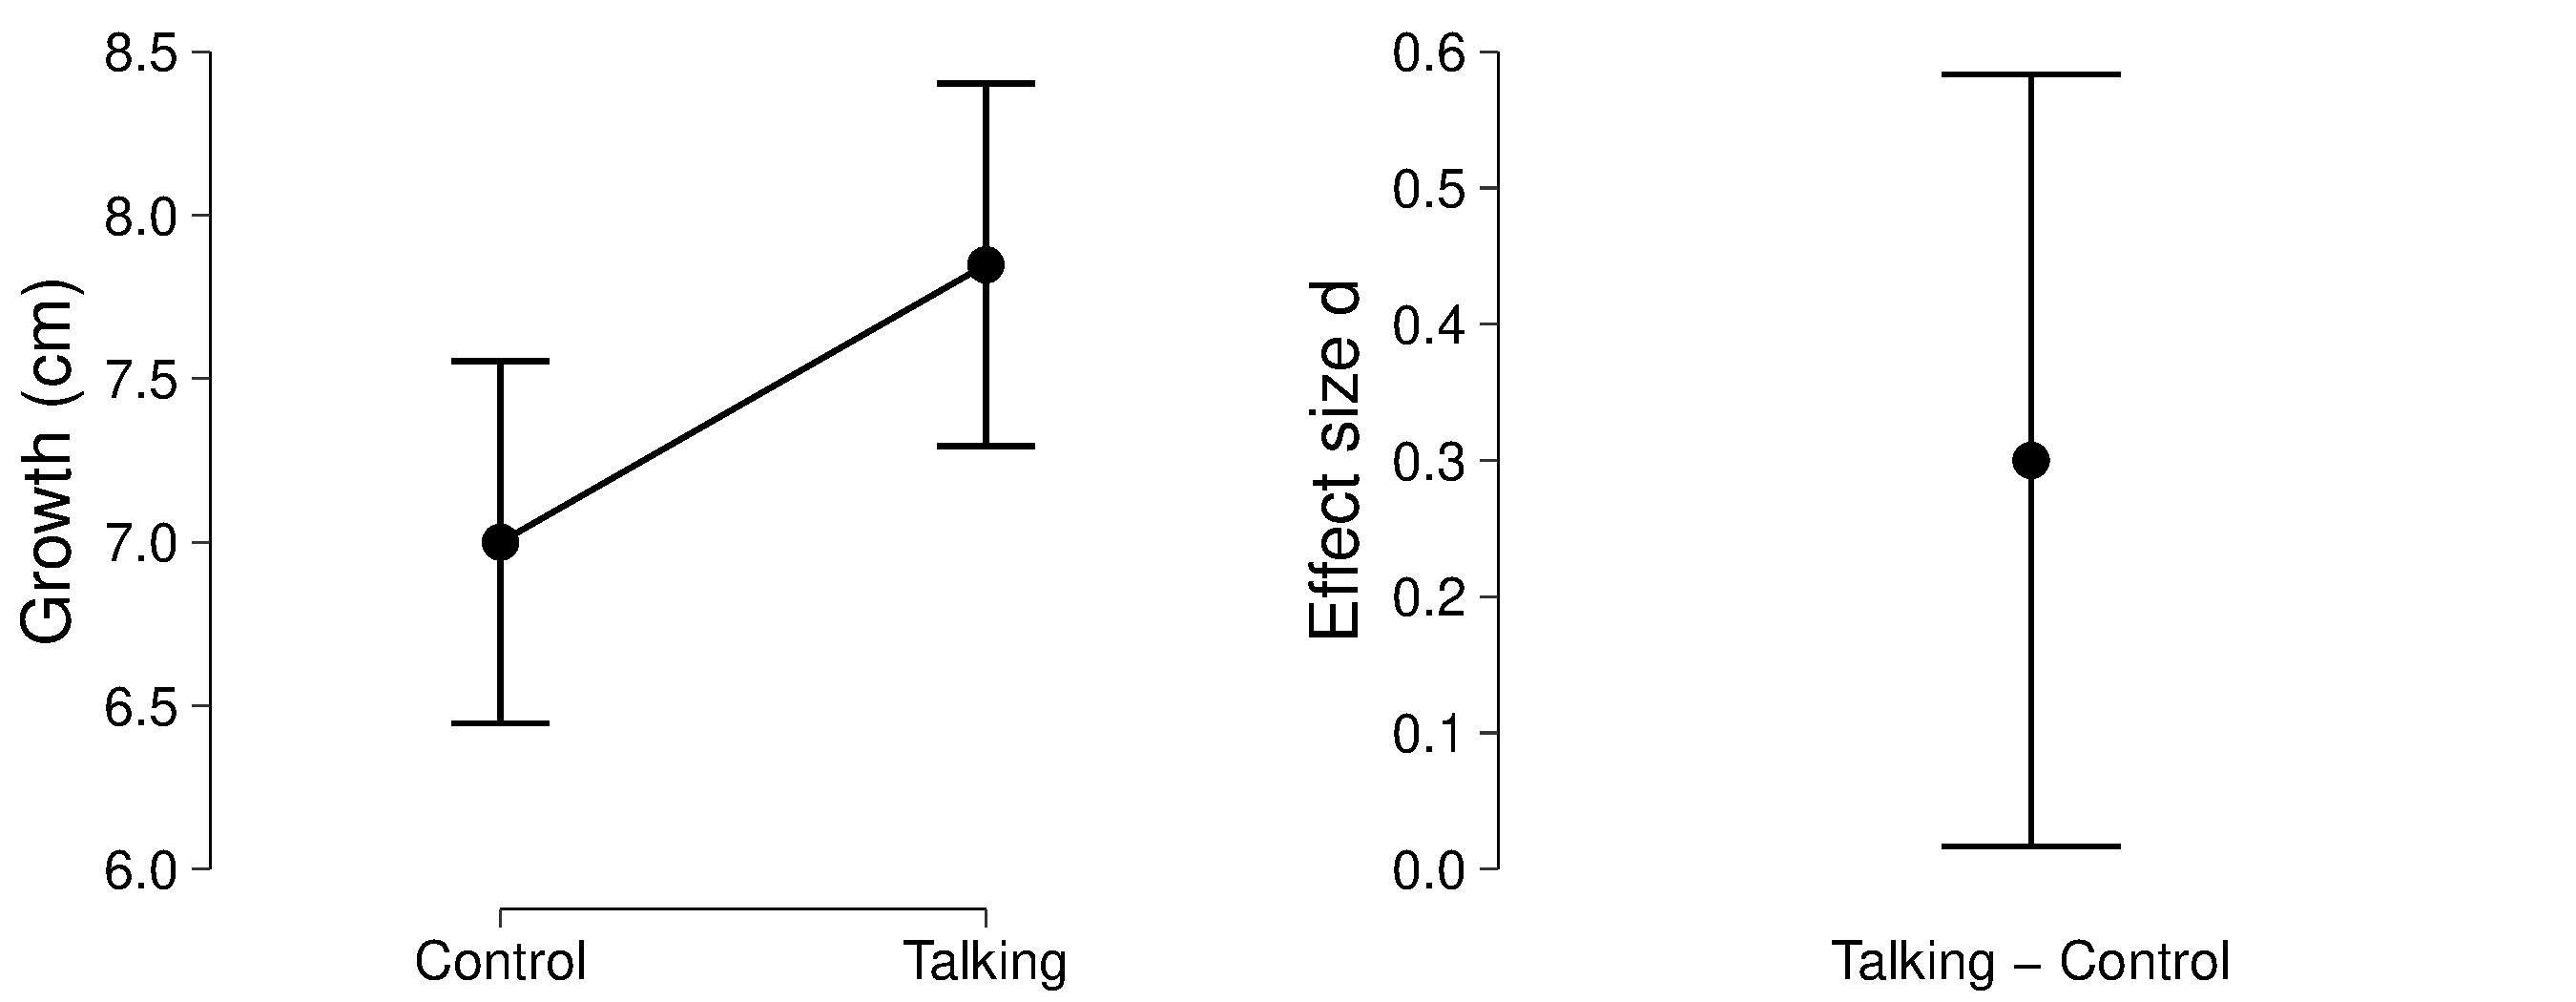
\includegraphics[width=\textwidth]{descriptivesPlot.pdf}
	\caption{The left panel shows a descriptives plot with the mean and 95\% confidence interval of the simulated plant growth. The right panel shows an estimate of the effect size, Cohen's \cohend, and a 95\% confidence interval.}
	\label{fig:descriptivesPlot}
\end{figure}
Given the results shown in Figure~\ref{fig:descriptivesPlot}, what is a reasonable point estimate of effect size? An straightforward answer is ``\getValue{0}{Estimate}{\tbEffectSizeExample}'' which makes intuitive sense from an estimation perspective.
%since the confidence interval does not contain 0, the sample effect size seems to be a reasonable choice. 
However, your colleague now tells you about the nature of the experiment: plants grow faster when you talk to them.\footnote{Specifically, imagine your colleague took 100 plants and measured their growth during three weeks. The first week 50 plants were randomly selected and spoken to while the other served as control. The next week, the roles reversed and the previously spoken to plants served as controls while the control plants were now talked to. The quantity of interest is the difference in growth between the weeks. This example is inspired by \protect\cite{BergerDelampady1987}.} Suddenly, an effect size of ``0'' also appears plausible.\footnote{Unless you talk out loud, with consumption, and the plant is near.}

%\section*{Why Confidence Intervals Overestimate Effect Size}
\section*{When is Effect Size Overestimated?}
Point estimates and confidence intervals of effect size based on only the alternative hypothesis tend to overestimate effect size. This overestimation is caused by the strong assumption that the null or perinull hypothesis is irrelevant. However, the null or perinull (ref Tukey\DONside{ref Tukey}) can have high plausibility after seeing the data. This happens when the prior odds in favor of a null effect are large (e.g., for a null hypothesis like ``Talking to plants has no effect on their growth.''), or when the data are so uninformative that after seeing the data there is substantial uncertainty about which model best describes the data. If the null hypothesis has a high posterior plausibility, it is obvious that it cannot be ignored, but that is exactly what is done when estimates are only based on the alternative hypothesis. As a result, the estimates are overconfident and, because the null hypothesis would shrink the estimates towards zero, overestimated.

\section*{A Bayesian Model-Averaged Perspective}
Here, we illustrate the overestimation and a remedy against it by reanalyzing the simulated data from Figure~\ref{fig:descriptivesPlot}.\footnote{Code for the reanalysis is available at \osflink{}.} We consider two hypotheses: The null hypothesis (\hypo{0}), speaking to plants does not make them grow faster or slower ($\cohend = 0$), and the alternative hypothesis (\hypo{1}), speaking to plants makes them grow faster or slower ($\cohend \neq 0$). We consider both these hypotheses using a paired-samples t-test. Typically, an estimate of effect size is based on solely the alternative hypothesis, which yields a point estimate and an uncertainty interval (for frequentists, $\cohend = \getValue{0}{Estimate}{\tbEffectSizeExample}$, 95\%  CI: \getCI{0}{\tbEffectSizeExample}; for Bayesians $\cohend = \getValue{1}{mean}{\reanalysis}$, 95\% CRI: \getCI{1}{\reanalysis}). %
\DONside{(Comment is too long, see the first page). Something is off with the Bayesian posterior mean in comparison to the frequentist ones. Both Jeff \& Julia and Bayesfactor seem to use $d = \mathrm{mean}(x-y)/\mathrm{sd}(x-y)$, but the R package uses $d = \sqrt{2}\mathrm{mean}(x-y)/\mathrm{sd}(x-y)$. The factor $\sqrt{2}$ seems crucial! if I add it the posterior means resembles the frequentist estimate, but the evidence is way too extreme. If I leave it out then the posterior mean appears too low although the obtained BFs are reasonable in comparison to the p-values. I did some small simulation studies, but this difference messes up the comparison so far (and ideally we use something existing for the frequentists CIs). I'm gonna look into the frequentist details on this.} 
However, it has been shown repeatedly that averaging over the models considered provides the best predictive performance (\citeNP[pp. 640--641]{ZellnerVandaele1975}, as described in \citeNP[p. 600--601]{ZellnerSiow1980}; \citeNP[p. 57]{Haldane1932}, \citeNP{IversonEtAl2010}, \citeNP{RouderEtAl2018PBR}), and conceptually similar ideas date back much further (\citeNP[p. 387]{WrinchJeffreys1921}, \citeNP{Jevons18741913}). Accordingly, our proposed remedy is to average across the null model and the alternative model, weighted by their posterior model probabilities.\footnote{For effect size, we obtain the following model-averaged posterior distribution: $p(\delta\midd\data) = s(\delta)pr(\model_0\midd\data) + p(\delta\midd\data,\model_1)pr(\model_1\midd\data)$. Here, $s$ is the Dirac delta function which represents the spike under the null, $pr$ denotes probability, and $p$ denotes density.} Figure 2 contrasts inference based on the alternative hypothesis with inference based on the averaged model by showing intervals and posterior means. 
%Figure~\ref{fig:modelAveragedPosterior} contrasts inference conditional on the alternative and inference conditional on the alternative model based on thefor shows for both the model averaged posterior and the posterior under the altnerative the posterior effect size under $\model_1$, their credible intervals, and their posterior means.
\begin{figure}[!ht]
	\centering
	\begin{tikzpicture}
		\node[anchor=south west,inner sep=0] (image) at (0,0) {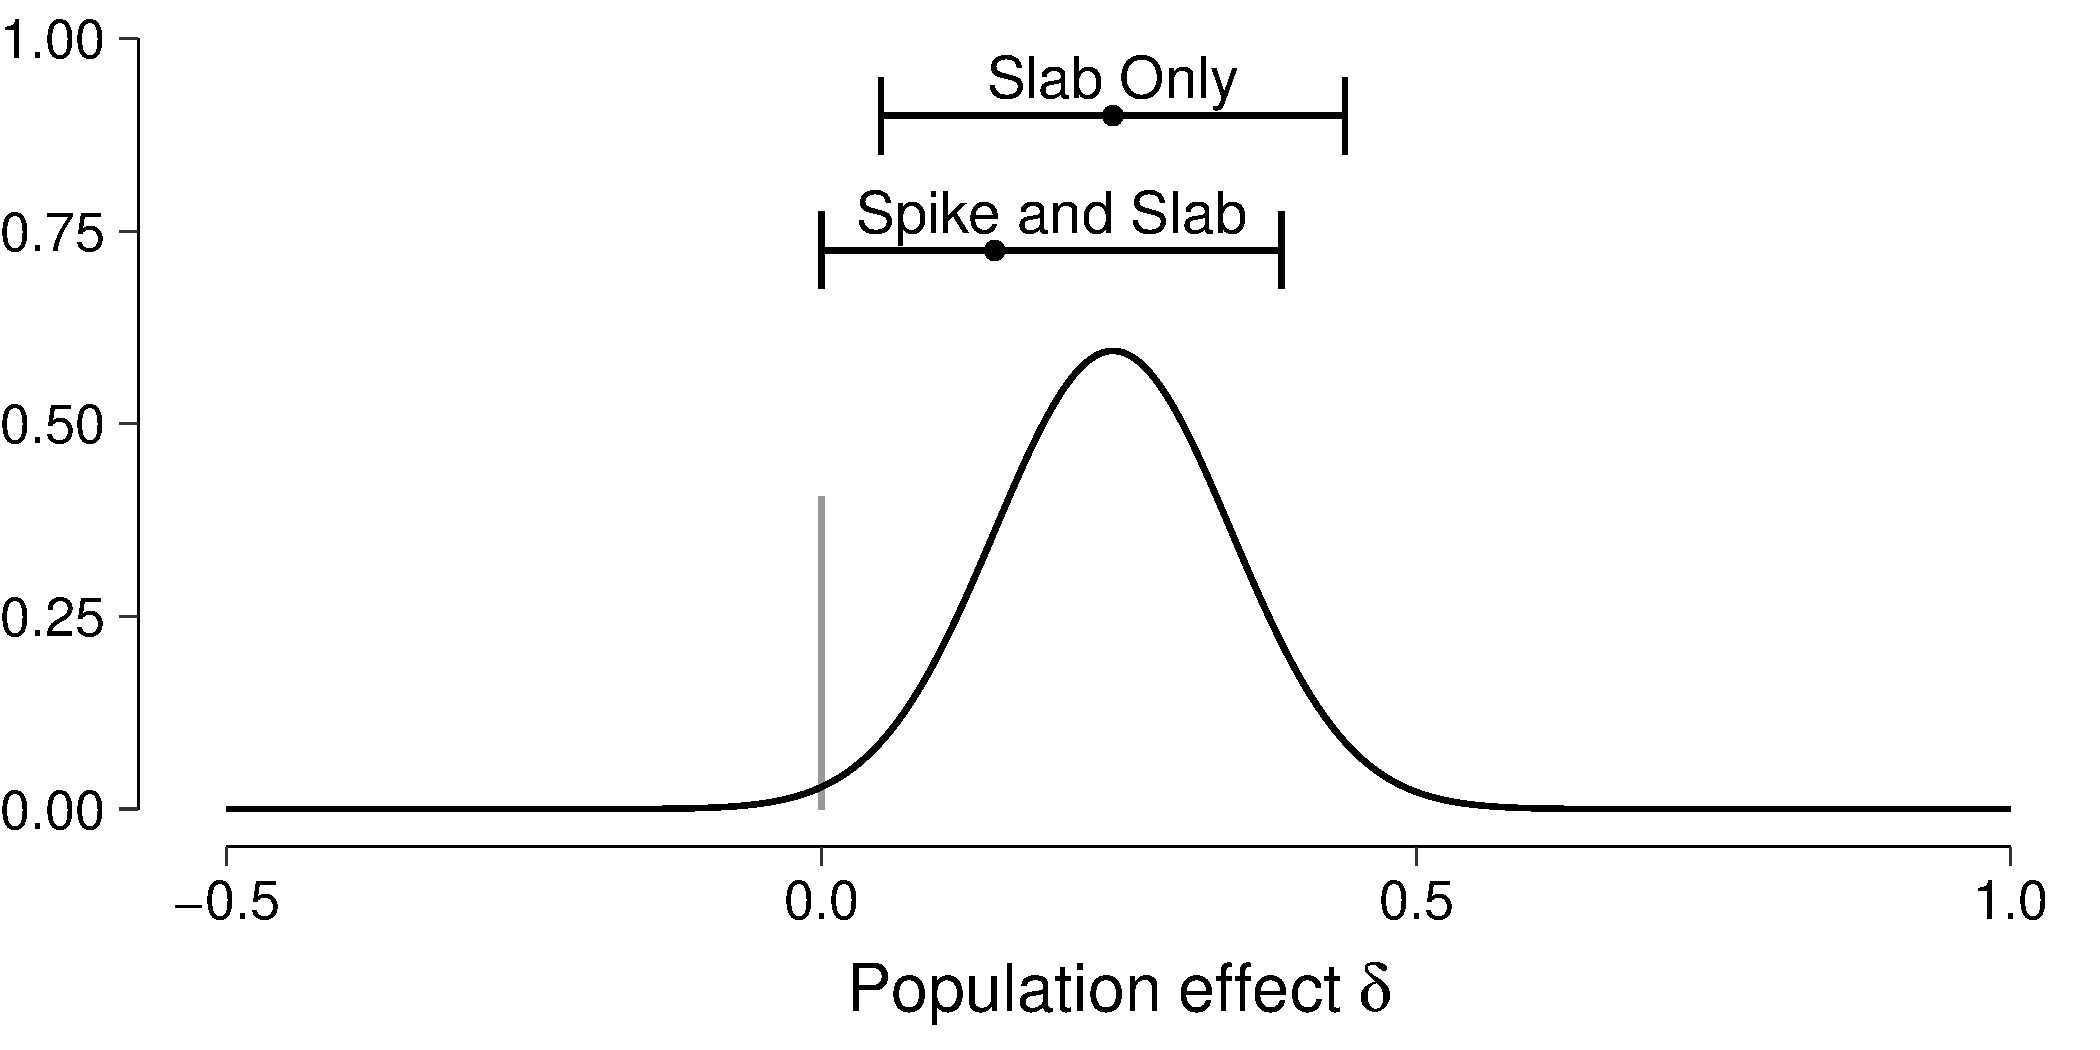
\includegraphics[width=0.9\textwidth]{spikeAndSlabPosteriorRescaledPosteriorMode.pdf}};
		\begin{scope}[x={(image.south east)},y={(image.north west)}]
		\node[anchor=base,inner sep=0pt, outer sep=0pt] at (0.24,0.55) {$p(\hypo{0}\mid\data) = \getValue{0}{ph0}{\reanalysis}$};
		\end{scope}
	\end{tikzpicture}
	\caption{A visualization of model averaging. The black line represents the posterior distribution of effect size given the alternative model (i.e., the slab). The posterior is scaled so that its mode equals the posterior probability of the alternative model. The gray line represent the posterior probability of the null model (i.e., the spike). The error bars and dots above the density show a 95\% credible intervals and the posterior mean for both the the slab and the model averaged posterior.}
	\label{fig:modelAveragedPosterior}
\end{figure}
The model averaged posterior mean and credible interval are shrunken towards 0 compared to the posterior mean conditional on the alternative hypothesis (\getValue{0}{mean}{\reanalysis} (95\% CRI: \getCI{0}{\reanalysis}) vs. \getValue{1}{mean}{\reanalysis} (95\% CRI: \getCI{1}{\reanalysis})). This makes sense as the posterior probability of the null hypothesis (\getValue{0}{ph0}{\reanalysis}) is non-negligible.

\section*{Discussion}
Here, we argued that estimates of effect size based on only the alternative hypothesis tend to be overconfident, in particular when a null or perinull hypothesis could also describe the data well. Consequentially, point estimates and confidence intervals based solely on the alternative overestimate effect size. A solution for this overestimation is averaging over the null and alternative hypothesis. Although this idea is not new, the influence of the null is still too often ignored in practice.

This approach contrasts with the popular estimation mindset, where it is argued that statistical significance should be abandoned in favor of estimation \cite{McShane2019abandon, Cumming2014}. Some may argue that all null hypotheses are false \cite{Cohen1994}\DONside{Double check ref Cohen}. However, there are statistical motivations to consider a point null \cite{BergerDelampady1987} and several large-scale replications studies have demonstrated that a near-zero effect size is reasonable in practice \cite<e.g., see the meta-analyses conducted by>{KleinEtAl2018ML2, CamererEtAl2018, NosekLakens2014}. The argument is not affected if the point null is replaced by a perinull.

A key aspect of model averaging is that it does not require model selection; there is no need to commit to a single model to obtain parameter estimates, although multiple models are considered. Therefore, model-averaged predictions and parameter estimates do fit the philosophy behind focusing on estimation. A skeptic might remark that in order to model average, it is necessary to obtain some form of model evidence and transform this into posterior model probabilities (e.g., Bayes factors, information criteria) which reintroduces the importance of testing. This could reintroduce the importance of testing as the method for obtaining model evidence has a large influence on the results. However, the same can be said for traditional estimation based inference, since confidence intervals can be constructed in multiple ways (e.g., bootstrapping, normal approximation). 

\subsubsection*{When not to model average}
When the sole aim is prediction rather than estimating and interpreting parameters, model averaging will likely be beneficial. However, if the goal is to interpret or base decisions on parameter estimates, there are several reasons to forgo model averaging. First, if the models are theoretical opposites it makes little sense to model average. The model-averaged parameters will be uninterpretable and thus meaningless. Second, the nature of the problem may be ill-suited for model averaging. For example, imagine we want to maximize patients' quality of life. A new experimental treatment, living at a high altitude for 2 years, will improve patients' quality of life but only if they stay for the entire 2 years. Providing patients with treatment essentially boils down to subsidizing their stay there for two years. For each patient, it is unknown whether they will complete the treatment or not. Here, one model represent that a patient finishes the treatment while another model represents that they do not. Using some background variables as predictors, we obtain for each patient the posterior probability that they complete the treatment. However, in this scenario it is meaningless to average the subsidy spent on a patient by the posterior probability of them completing the treatment, as such an average would always provide patients with less than the required amount to complete the treatment, essentially wasting the subsidy. More generally, whenever some form of thresholding will be applied to the model outcomes, results of model averaging may not be useful.

In sum, we argue that descriptions of effect size based on only the alternative hypothesis are overconfident and as a consequence overestimate effect size. A remedy for this overestimation is model averaging. Although this idea is not new, model averaging remains underutilized in practice and we hope this paper brings more attention to model averaging.

\bibliographystyle{apacite}
\bibliography{referenties, referenties.bib}
%\clearpage

%\appendix
%\counterwithin{figure}{section}
%\begin{figure}[!ht]
%	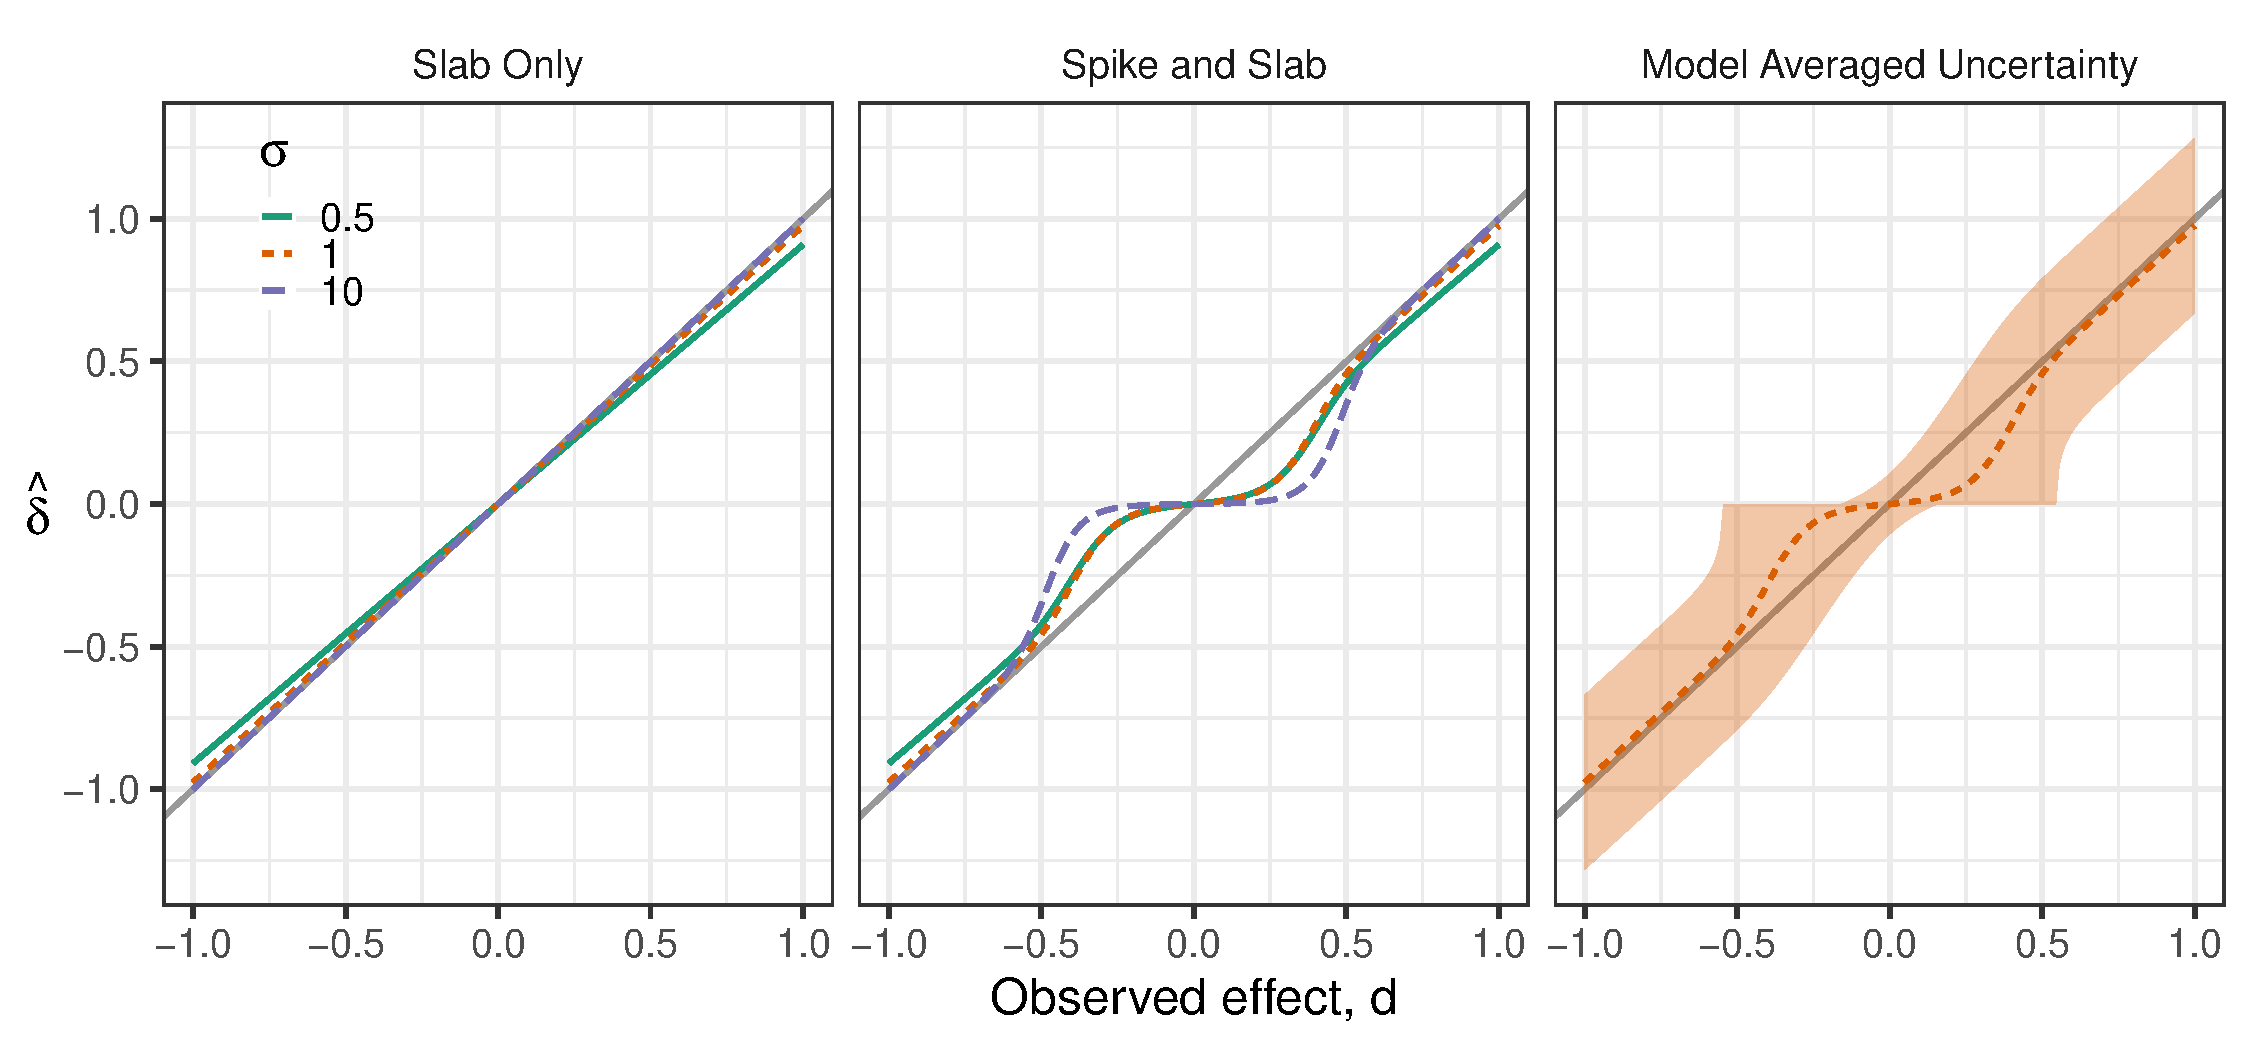
\includegraphics[width=\textwidth]{posteriorMeanVsSampleDelta3panel.pdf}
%	\caption{Posterior mean for effect size (y-axis) as a function of the observed effect size (x-axis). The left panel shows inference conditional on the alternative model (i.e., the slab). The middle panel shows the model averaged posterior mean, which shrinks towards 0 as the sample effect size approaches 0 and the null model becomes more plausible. The right panel shows the a 95\% credible interval for the model averaged posterior. The colors and line types represent different variances of the prior distribution.}
%	\label{fig:posteriorMeanVsSampleDelta}
%\end{figure}


% comment graveyard

%With sparse data, the prior distribution shrink the estimate towards its mean, in this case 0.\DON{I know the prior shrinks estimates towards 0, but this has little to do with the true effect size. Rather, it's a reason why Bayesian estimators (of effect size) are be biased and tend to underestimate the true value.}
% In addition, since the null hypothesis is considered a-priori plausible, its predictions should be considered also. It has been shown repeatedly that model averaging provides the best predictive performance (\citeNP[pp. 640-641]{ZellnerVandaele1975}, as described in \citeNP[p. 600-601]{ZellnerSiow1980}; \citeNP[p. 57]{Haldane1932}, \citeNP{IversonEtAl2010}, \citeNP{RouderEtAl2018PBR}), and conceptually similar ideas date back much further (\citeNP[p. 387]{WrinchJeffreys1921}, \citeNP{Jevons18741913}). Thus, to obtain the best predictions one should model average over the null and alternative hypothesis. The impact of the null will shrink the estimate of effect size towards 0.
% 
% \J{We should probably first introduce the two relevant models here, and the idea that an unconstrained model is used for estimation. Maybe even say something like noone would use the null model to generate effect size estimates, why would we use the unconstrained?}

%\DONside{Let d be the effect size of the model averaged posterior predictive distribution. Consider the limit of d as the number of posterior predictive observations goes to infinity. Do we retrieve the model averaged posterior effect size? Intuitively yes, which could be a nice argument that the model averaged effect size can definitely be interpreted for this model.}

%Show prior-posterior plot from JASP:
%With sparse data, the prior distribution on effect size will shrink the estimate towards 0. Happens with the default settings, but even more when the width is smaller.
%
%Also, show spike at zero (maybe we need better JASP plot, will ask Don to create it):
%
%The impact of H0 will shrink the estimate toward 0. This is most clear when H0 is a priori very likely (''plants do not grow faster when you pray for them'') or when the sample effect is very close to zero, so that it becomes clear that H0 might provide a more reasonable explanation.
%
%Mention earlier literature:
%Model averaging effect size:
%\cite[pp. 640-641]{ZellnerVandaele1975}, as described in \cite[p. 600-601]{ZellnerSiow1980}; also \cite[p. 57]{Haldane1932}, \cite{IversonEtAl2010}
%
%Early ideas that are conceptually similar can be found in \cite[p. 387]{WrinchJeffreys1921} (show BMA between $\mathcal{H}_1$ and $\mathcal{H}_0$ -- but for prediction, not estimating effect size!; see also \cite{Jevons18741913}).
%
%See also \cite{RouderEtAl2018PBR}:
%
%Key is Figure 5. The spike-and-slab model shows shrinkage towards zero for small observed effect sizes because the spike has increased influence.
%
%``There are alternative interpretations that we find somewhat cumbersome. One is that the spike-and-slab can be viewed not as a model but as a model-averaging device. Here, the goal is not so much to define categories of effect and no-effect, but to average across both of them, and this averaging results in regularization. If one uses this interpretation, the prior odds settings are important as they influence the posterior weight given to each model component in the averaging. Another alternative interpretation comes from Kruschke and Liddell (Kruschke, 2011; Kruschke \& Liddell, 2017; this issue). Here, the spike and slab are seen as separate components in a hierarchical model. Accordingly, a focus on Bayes factors denotes a focus on the choice between components; a focus on posterior estimation entails parameter estimation after choosing the slab. We find this view difficult inasmuch as there is no a priori reason to choose the slab to focus on estimation. If one admits the possibility of the spike, then assuredly it should affect posterior estimation as well.''

%There are at least two reasons for this tendency to overestimate. The first reason is that there is a high base-rate of null effects which leads to high prior odds in favor of a null effect. The second reason is that when the data are not very overwhelming, the posterior plausibility of a point null can be large. This implies that the null should not be ignored, but this is precisely what happens when inference is based only on the alternative. These reasons originate from the unheeded assumption that a null or perinull hypothesis is irrelevant and lead to overconfident estimates and intervals. Since ignoring the null hypothesis effectively avoids shrinkage towards 0, this overconfidence is associated with an overestimation.
\end{document}